\section{Introduction}

%\par{Machine learning systems automatically learn programs by training and analyzing a large number of data in real time or offline, in order to obtain regular knowledge or predict the future data. Machine Learning has become an important way to enhance the accuracy of decision-making for various industries include Web search, spam ?lters, recommender systems, ad placement, credit scoring, and many other applications \cite{alpaydin2014introduction}, \cite{ZhihuaZHOU2016introduction}, \cite{bengio2009learning}. The existing distributed computing framework models the computational process of the machine learning algorithm as the state transitions between key-value pairs such as MapReduce\cite{dean2008mapreduce}, spark \cite{zaharia2010spark} and so on.}

Key value grouping operation, known as GROUP BY clause, is a key operation in traditional data management systems \cite{gray1997data}, \cite{stephens2005oracle}, \cite{mysql2009mysql}, \cite{momjian2001postgresql}. It groups a set of out-of-order records into multiple groups according to a certain key. GroupBy operation is often used with aggregate functions which produces a single row of summary information for each group, e.g., GroupBy-Aggregate in SQL. GroupBy is also widely used in distributed computing frameworks for processing big data. MapReduce \cite{dean2008mapreduce} expresses the computational process as three phases: Map, Shuffle and Reduce. During shuffle phase, key-value pairs that have the same key are aggregated together to form the Map output file so that a group of intermediate key-value pairs with the same key are sent to the same Reduce processor where the final cluster-wide aggregation (reduction) is applied on them. The efficiency of key grouping step is essential both in relational databases and in distributed computing frameworks.
%\par{All the out-of-order key-value pairs are aggregated together according to the same key, The aggregating process is called key value grouping . The key-value grouping is widely used in both distributed computing framework and traditional relational database \cite{stephens2005oracle}. MapReduce expresses the computational process as three phases: Map, Shuffle and Reduce. During shuffle phase, The key-value pairs which have the same key are aggregated together to form the Map output file so that groups with the same key will be send to the same Reduce processor. In relational database, The SQL(Structured Query Language) GROUP BY is generally used in a SELECT statement to collect data across multiple records and group the results by one or more columns. The SQL executes the GROUP BY clause by using key-value grouping, the columns are specified by the user followed by GROUP BY can be regarded as the key, and the remaining columns can be used as values.}

\textcolor {red}{Another popular use case for key grouping is to accumulate state across the stream in distributed stream processing engines (DSPEs) such as Storm \cite{storm2013storm}, S4 \cite{neumeyer2010s4}, Smaza \cite{noghabi2017samza}. This grouping in DSPEs is usually implemented by partitioning the stream on a key \cite{nasir2015power}. The strategies that are used to route tuples in a stream toward available operators can be divided into two categories: key grouping for stateful operators where a stream of tuples is partitioned in several disjoint sub-streams depending on the values contained \cite{rivetti2015efficient} and shuffle grouping for stateless operators where each tuple of a stream can be randomly assigned to any available operator \cite{Rivetti2016Online}. However, all the above works are focused on how to route kv-pairs to available operators for alleviating load imbalance but ignoring local key value aggregation overhead at the receiver side. In fact, the execution time depends on not only stream partition but also local aggregation. Our work will focus on accelerating the local GroupBy aggregation in this paper.}

There are two categories of GroupBy implementations in general, sort-based grouping and hash-based grouping. Basically, the \textbf{sort-based grouping} makes the set of data records sorted in the order of the group key, so that the records with the same group key are located together. While the \textbf{hash-based grouping} typically hashes key-value pairs to a hashtable structure where multiple key-value pairs in the same group (sharing the same group key) are stored in the same bucket.

A few variations of both sort-based grouping and hash-based grouping exist. Recall that key-value pairs (kv-pairs) grouping operation is the key operation in Hadoop MapReduce \cite{dean2008mapreduce}. The map output kv-pairs are locally grouped by keys before shuffling to reduce workers. These map output kv-pairs (i.e., reduce input kv-pairs) from various map workers are further merged to obtain a global grouped kv-pairs. Each group of kv-pairs sharing the same key is the input of a reduce function. In Hadoop Mapreduce implementation, a kind of sort-based grouping, \emph{merge-sort grouping}, is used, which can perform quite general grouping tasks at scale even in the absence of available memory. However, merge-sort grouping involves large amount of redundant computation and I/Os. The previous work \cite{shvachko2010hadoop,yu2009distributed,Li2011A} shows that merge-sort grouping adopted by Hadoop is found to be among the worst-performing choices. \textcolor {red}{Veselin et al. presents SYMPLE \cite{Raychev2015Parallelizing}, a system for performing MapReduce-style groupby-aggregate queries which parallelizes these user-defined aggregations by breaking dependencies using symbolic execution. However, the programmers have to learn to use SYMPLE��s symbolic data types.} For many applications, hash-based grouping improves performance because these applications require only unsorted grouping \cite{lin2011tenzing}, \cite{yu2009distributed}. However, hash-based grouping consumes more memory than sort-based grouping because it requires to load all records into memory. The performance heavily depends on the amount of available memory.

%merge-sort is applied both for the Map and Reduce phases to group key value pairs. The resulting systems can perform quite general grouping tasks at scale even in the absence of available memory, but using Mixed Sort offers a low-level grouping method and contains a mount of redundant computation, as the previous work shows that GroupBy implemented by Hadoop \cite{shvachko2010hadoop} are found to be among the worst-performing choices \cite{yu2009distributed}. For many applications, hash-based grouping improves performance because these applications require only unsorted grouping \cite{lin2011tenzing}, \cite{yu2009distributed}. However, hash-based grouping will consume more memory than sort-based grouping because it accumulates all the records in memory before performing any aggregation. The execution efficiency heavily depends on the amount of available memory, insufficient memory will limit the amount of data can be grouped of hash-based grouping and even cause the task to fail.

%����ʦָ��������1
%\textcolor{red}{please introduce merge-sort (mapreduce implementation),sql implementation, CBT, etc... list their pros and cons by considering performance and memory efficiency, and introduce figure 1.}

SQL databases mainly use sort-based grouping and some of them propose a hash-based grouping algorithm \cite{MySQLGROUPBYOptimization} \cite{Bratbergsengen1984Hashing}. The sort-based grouping is similar to that in Hadoop MapReduce. The default sort-based method is not the most efficient way to execute the Group By query \cite{mysql2009mysql}. A hash-based grouping has been used in MariaDB \cite{bartholomew2012mariadb}, Oracle \cite{stephens2005oracle}, Postgresql \cite{momjian2001postgresql}, and SQL Server \cite{agrawal2005database}. The hash-based grouping creates an in-memory hash table for grouping rows. If the hash table becomes too large to be fit in memory, the input records are partitioned into smaller work tables which are recursively partitioned until they fit into memory. Once all input groups have been processed, the completed in-memory groups are output and repeat the algorithm by reading back and aggregating one spilled partition at a time until all partitions have been processed. We refer to this approach as \emph{memory-constraint hash grouping}. It excels at efficiently aggregating large data sets and performs better than merge-sort grouping in some situation. However, when processing highly skewed data sets, the sub-tables sizes are not balanced, which leads to multiple recursive partitions and downgrade grouping performance.

introduce grouping and its importance

The state-of-the-art memory-constraint grouping includes 1. merge-sort, 2. repeat hash, 3. grouped hash, 4. indexing+filing, 5. ... (introduce them respectively). 

As known, in real life application, the group size exhibits power-law distribution. We observe that these grouping implementations exhibit different performance and memory cost for big groups and small groups. As shown in Figure. 1a, ..... So, for big groups, the best is indexing+filing. As shown in Figure. 1b, .... So the best for small groups is grouped hash. Therefore, the ideal implementation should take the group size into account, and a hybrid grouping approach is desired.

Two problems are raised. 1. How to detect the group size efficiently? 2. How to define big group and small group? 

For the first problem, we solve it by leveraging min-count sketch...

For the second problem, we formalize it as an optimization problem and solve it (obtain the optimal threshold that separate big and small groups) given the memory budget. 

We evaluate our algorithm through extensive experiments. Our results show that ....

The paper organization







In this paper, we propose an I/O efficient external hash grouping scheme \emph{bHash} that leverages both hashing and sorting. Basically, bHash contains two phases and needs to pass the input kv-pairs file twice. In the first phase, it hashes the kv-pairs in a hash table but only records the compressed group key and accumulates the value size that belongs to the same group key, by which we obtain the global data distribution knowledge, i.e., $\langle group key, group size \rangle$ information. With this knowledge, we assume the sorted file structure and compute every group's output position in the sorted file. Actually, we do not really sort but only guarantee the kv-pairs in the same group to be locate together. Given the size information of every group, the output file position (i.e., file offset) can be calculated by accumulating the group size. Then a table called \emph{pos\_table} that contains the global $\langle group key, file position\rangle$ information is obtained. In the second phase, using the in-memory buffered pos\_table, bHash needs another pass of the input file and outputs kv-pairs to file in terms of the pos\_table. Furthermore, in the second phase we provide an output buffer design that can greatly reduce the number of write I/Os. The ``b'' in bHash indicates both the buffered pos\_table and the output buffer, with the usage of which we can improve our performance a lot. To sum up, bHash benefits from both the \emph{hash} table's random access ability (from hash-based grouping) and the \emph{sorted} structure's sequential access ability (from sort-based grouping). With the buffer design, we can connect the hash table structure and the sorted structure and achieves a better performance.


%based on offset (bHash) leveraging the ��frequency statistics�� [14], and hash. The algorithm counts the frequency for each group, the kv-pairs will be directly mapped to the location in the grouping result file without sorting. Instead of storing kv-pairs in memory, bHash only stores the grouping key and the offset for each group in memory to reduce memory consumption. Because of the disorder between different groups, a large number of redundant overhead brought about by Mixed Sort grouping algorithm is eliminated. Our algorithm achieves a significant improvement on both performance and memory efficiency over a state-of-the-art, the bHash is described in Section 3.

\begin{figure}%figure 1
\label{fig:compare}
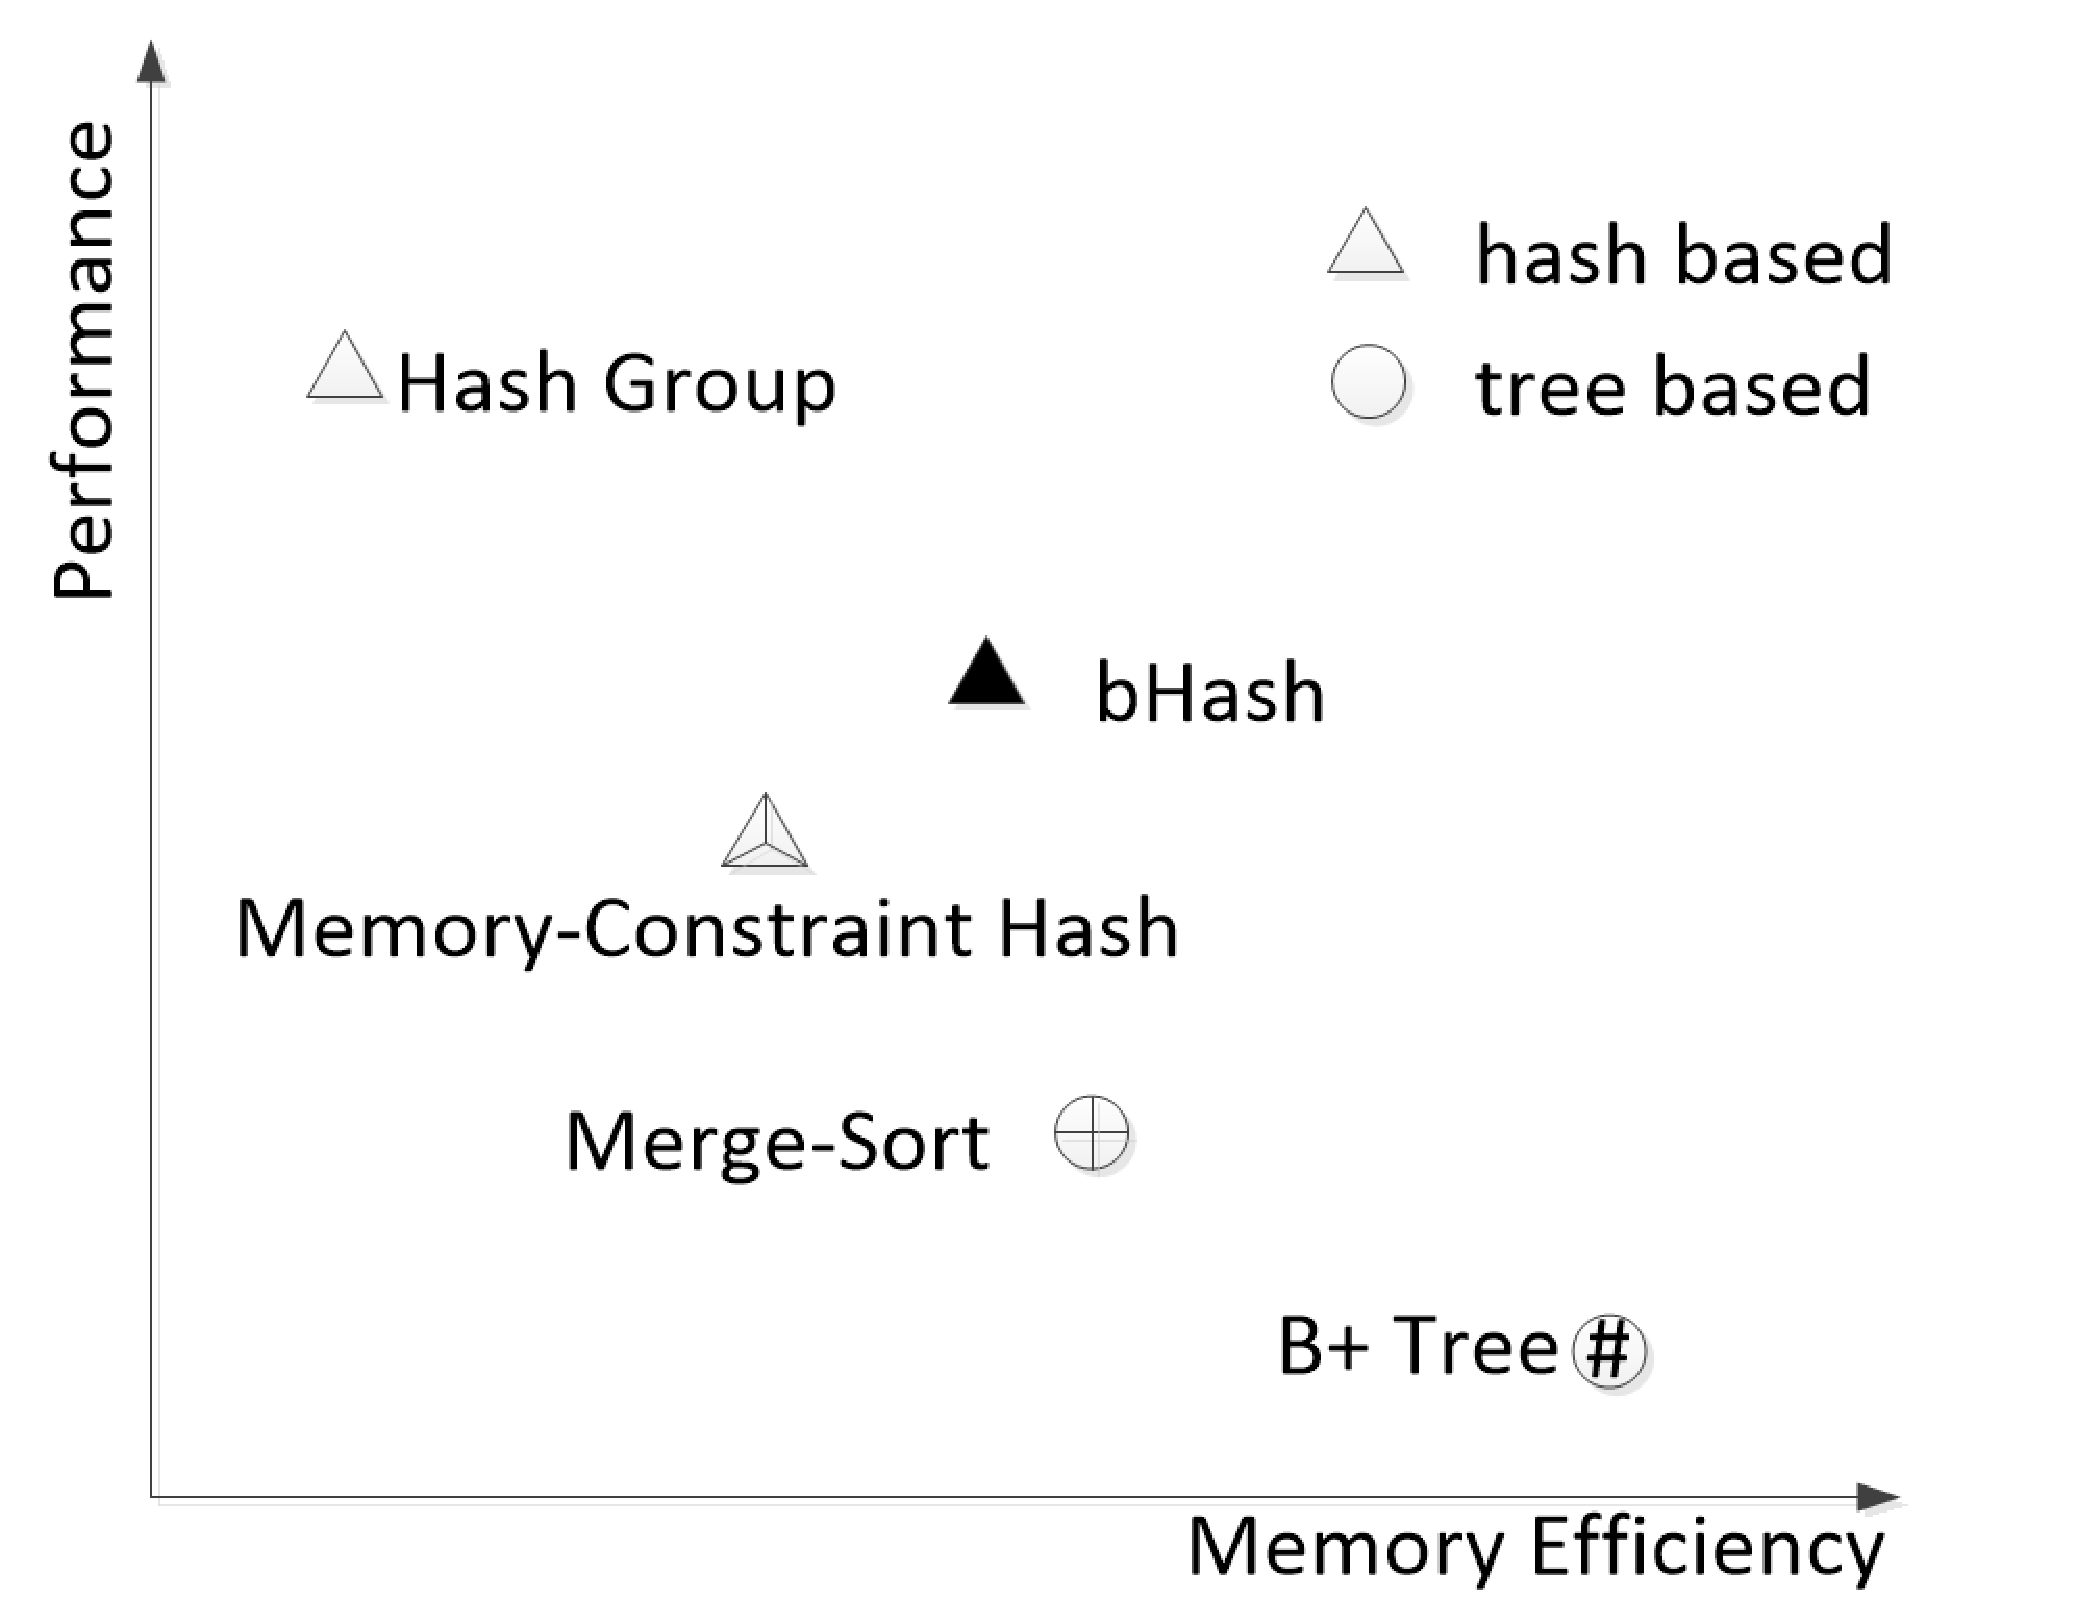
\includegraphics[width=2.5in]{fig/ComparisonPerformance}
\caption{Performance comparison of existing grouping algorithms.}
\end{figure}

Figure 1 presents a comprehensive comparison among various grouping algorithms in two dimensions, performance dimension (y-axis) and memory efficiency dimension (x-axis). If the memory size is large enough to fully accommodate all kv-pairs, the pure hash table approach is the fastest one (i.e., highest performance). At the other extreme, a sort-based grouping using B+ Tree structure to maintain the sorted kv-pairs is the most memory efficient approach which only requires page-size memory. For sort-based grouping, the merge-sort grouping requires more memory (lower memory efficiency) to improve performance. For hash-based grouping, memory-constraint hash grouping sacrifices performance for memory efficiency. Our bHash grouping algorithm only requires small size of memory to store the group size information and only requires two passes of the input kv-pairs to complete grouping. Therefore, it is endowed with both performance and memory efficiency.
%Thus, the memory consumption is the most. If the memory available just holds all key value pairs without extra space to resolve the hash collision, the Tree Sort in memory is the best method. Tree Sort does not require additional auxiliary space so the memory efficiency is better than Hash Group. For massive data, the Mixed Sort is a generalized method for limited memory. It quick sorts every chunk in memory and finally merge sorts these partial sorted chunks. The Mixed Sort slightly sacrifices performance to improve memory efficiency. In more extreme cases of larger data size, the LSM Tree and B+ Tree based on disk are relatively appropriate grouping algorithms to reduce memory usage but perform poorly. Hash-based algorithms such as CBT can not slove the case of inefficiency memory, the other Hash GroupBy algorithm in SQL databases better balances the memory efficiency and performance, but does not perform  well enough for skewed workloads.
%Applications of key-value grouping, especially in data mining and machine learning, typically require aggregating key value pairs across stream by grouping the data on specified fields \cite{alpaydin2014introduction}, \cite{ZhihuaZHOU2016introduction}. In MapReduce, this grouping is usually implemented by Mixed Sorting the data on a key and ensuring that messages with the same key are aggregated together and processed by the same Reduce. Typically, it first maps continuously arriving key pairs to memory buffer constantly, then quick sort and spill these key-value pairs to the disk when the amount of cached data has reached the upper limit of buffer. Commonly, the total quantity of data far exceeds the size of the memory buffer, so there will be multiple internal sorted files spilled to the disk. Because the key range covered by these spilled files overlaps, a merge sort is required to generate the final grouping file. Finally, all key value pairs that have the same key are aggregated together by Mixed Sorting. The Mixed Sort grouping does not depend on the data distribution and is scalable. Alas, it also brings about redundant computation overhead as it represents a ��fully sorted�� paradigm. It disregards the non-necessity of key ordering among different groups, i.e., there is no need to maintain the grouping key order between two groups , for example, the data in group one must be followed by group two just because the key of group one is smaller than that of group two. Actually, the only thing we want to do is to bond these key-value pairs have the same key together, and not to care about the relative location of different grouping key value pairs, as depicted in Figure 2.

%\par{Large web companies run massive deployments of data mining or machine learning in production. Given their scale, good utilization of the resources and improving computation efficiency is critical \cite{nasir2015power}.  However, the Mixed Sort algorithm involves a large number of sorting calculation among different groups, which brings a lot of redundant computing overhead and seriously affects the efficiency of the algorithm.}



%\par{On the other hand, grouping key value is also applied in traditional relational database. SQL databases use two entirely different grouping algorithms, the sort/group algorithm and the hash algorithm. When the user calls the GROUP BY clause, MySQL also mixed sorts by default to group records, which means using ��File Sort�� \cite{MySQLGROUPBYOptimization}. File Sort operator reads its input into memory, sort in memory and outputs the sorted result. If there is Limited memory available, it merge sorts the remainder of the input using an indexed-based sort method. The performance is affected by the size of the key to sort, the row size, and the total size of input records. The default sort/group method isn��t the most efficient way to execute the Group By query \cite{mysql2009mysql}. A new hash group by method has been proposed in MariaDB \cite{bartholomew2012mariadb}, Oracle \cite{boicea2012mongodb}, \cite{momjian2001postgresql}, and SQL Server \cite{agrawal2005database}. The hash group by algorithm creates an in-memory hash table for grouping rows. As rows are read from input, the grouping rows are updated. If the hash table doesn��t fit into memory, the input records are partitioned into smaller work tables which are recursively partitioned until they fit into memory. Once all input groups have been processed, the completed in-memory groups are output and repeat the algorithm by reading back and aggregating one spilled partition at a time until all partitions have been processed. The hash group by algorithm excels at efficiently aggregating large datasets, and performs better than File Sort algorithm in some situation. However, when dealing with skewed data sets, the partition size is uncertain , which leads to the algorithm need to repeat many times. Repeatedly reading and writing disk will brings a lot of I/O overhead.}
%����ʦָ��������2
%\textcolor{red}{please do not mention machine learning framework. we don't need to motivate our work in that way. groupby is a fundamental operation in database, this is a wellknown problem. To better motivate our approach is that we need to find the fundamental limitation of current approaches and propose to address that unique limitation. You can write first and let's discuss.}

%\par{In this work, we focus on the problem of key value grouping in machine learning computing framework and SQL GROUP BY operator. Machine learning algorithms usually iterate repeated and constantly update training parameters, the high execution efficiency of key value grouping is required especially when the input data set is massive even follows a skewed key distribution \cite{Mahout}. On the other hand, SQL query efficiency is also very important, such as the GROUP BY clause. The default Mixed Sort method is a resource-intensive operation and performs not well enough. Furthermore, the other improved hash group by algorithm cannot cope with data skew disaster.}


 %While key value pairs are generated , a frequency hash table is established in memory. Every entry keeps the grouping key and the number of corresponding key value pairs seen by now, and the frequency of different groups will be updated constantly with the arrival of key value pairs. The hash bucket is partitioned horizontally to divide the source key value file into a plurality of small files, so as to reduce the range of key covered by each sub source file. Then, the grouping frequency hash table in memory is converted to a grouping offset hash table. Read each key value pair from sub source file, the final offset in grouping result file can be obtained by searching the grouping offset hash table in constant time and then the key value pair is stored directly on the predicated location in the result file. Once a key value pair has been output, the offset of its group increases one.}
%
%\par{A first issue is how to traverse the frequency of variable�Clength key value pairs to offset.  For fixed-length key value pairs, the offset of the current key value pair equals to the sum of the offset of the previous key value pair and the product of its frequency and the byte-occupancy of the fixed type. Instead, we propose that each hash entry keeps the byte occupancy of one group to deal with variable�Clength key-value pairs. In this paper we prove that, interestingly, a simple offset counting method, whereby each hash entry independently tracks the size of one group, performs very well in practice.}

%The combination of these two techniques (hash and frequency counting) enables a new key-value grouping scheme named Hash Key-value Grouping Based on Offset (bHash).
Our main contributions can be summarized as follows.

\begin{list}{\labelitemi}{\setlength{\leftmargin}{5mm}\setlength{\itemindent}{0mm}
\setlength{\topsep}{0.5mm}\setlength{\itemsep}{2mm}\setlength{\parsep}{0mm}}
\item Firstly, we study the problem of key grouping in modern distributed processing engines and traditional relation databases.

\item Secondly, we present an I/O efficient external hash grouping scheme that leverages both hashing and sorting., which employs the combination of hash technique and data distribution statistics  and eliminates the computational overhead of inter group ordering in the case of using less memory. %bHash scales almost linearly to $O(n)$.
    We also analyze the performance and memory efficiency.% of the algorithm is proved theoretically and practically.

\item Thirdly, we evaluate bHash on both real data sets and synthetic data sets. Compared to the existing key grouping algorithms including merge-sort and memory-constraint hash, bHash improves the performance by 20\%-57.8\% with the same memory usage. For the long-tailed distributions, our algorithm achieves 50\% better overall performance than merge-sort but takes up 40\% times less memory. It is also 45\% faster than memory-constraint hash with 39\%times less memory.
\end{list}

The rest of this paper is organized as follows. Section \uppercase\expandafter{\romannumeral2} describes the related work. In Section \uppercase\expandafter{\romannumeral3}, we propose our grouping method bHash and present the key optimizations. Section \uppercase\expandafter{\romannumeral4} discusses the parameters setting. The experimental results are presented in Section \uppercase\expandafter{\romannumeral5}. Finally, Section \uppercase\expandafter{\romannumeral6} concludes the paper.
%\begin{figure}
 % \centering
  % Requires \usepackage{graphicx}
  %\includegraphics[width=.5\textwidth]{cats.png}
 % \caption{Performance comparison of existing grouping algorithms.}
 % \label{referencename};
%\end{figure}
